\documentclass[]{report}
\usepackage{amsmath}
\usepackage{amssymb}
\usepackage[english]{babel}
\usepackage[utf8]{inputenc}
\usepackage[T1]{fontenc}
\usepackage{euler}
\usepackage[inner=0cm,outer=0cm,top=0.1cm,bottom=0cm,paperwidth=8cm,paperheight=5cm]{geometry}

\usepackage{chemfig}
\usepackage{tikz,pgfplots}
\usetikzlibrary{positioning}
\usetikzlibrary{decorations.pathmorphing}

\renewcommand*\printatom[1]{\ensuremath{\mathsf{#1}}}

\definecolor{myyellow}{RGB}{255,214,0}

\begin{document}
\centering
	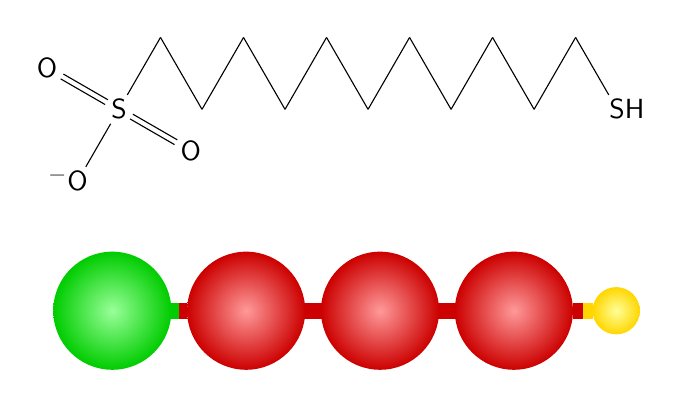
\begin{tikzpicture}
		%\draw[gray,step=1] (-5,-3) grid (5,3);
		\node at (0,1) {\chemfig{^{-}O-[:60]S(=[:-30]O)(=[:150]O)-[:60]-[:-60]-[:60]-[:-60]-[:60]-[:-60]-[:60]-[:-60]-[:60]-[:-60]-[:60]-[:-60]SH}};
		
		\draw[line width=2mm,-,black!20!red] (-1.2,-1.5) -- (2.2,-1.5); 
		\draw[line width=2mm,-,black!20!red] (2.95,-1.5) -- (3.075,-1.5);
		\draw[line width=2mm,-,myyellow] (3.075,-1.5) -- (3.2,-1.5);
		\draw[line width=2mm,-,black!20!green] (-2.15,-1.5) -- (-2.05, -1.5);
		\draw[line width=2mm,-,black!20!red] (-2.05,-1.5) -- (-1.95, -1.5);
		\shade[outer color=black!20!green, inner color=green!40] (-2.9,-1.5) circle (0.75);
		\shade[outer color=black!20!red, inner color=red!40] (-1.2,-1.5) circle (0.75);
		\shade[outer color=black!20!red, inner color=red!40] (0.5,-1.5) circle (0.75);
		\shade[outer color=black!20!red, inner color=red!40] (2.2,-1.5) circle (0.75);
		\shade[outer color=myyellow, inner color=yellow!40] (3.5,-1.5) circle (0.3);
	\end{tikzpicture}
\end{document}
